\setchapterpreamble{
    \lettrine{T}{wo}~analyses are presented in this thesis: the first is an analysis of the branching fractions of~\BsDsK and~\BdDsK (\cref{chp:DsK_BF}), while the second is a measurement of the \CP-violation parameter~\CPgamma using the decay time of \BsDsK~events (\cref{chp:BsDsK_TD_Data,chp:BsDsK_TD}).
    Several experimental methods are common to these analyses: a loose event preselection (\cref{sec:stripping}), the use of multivariate methods to discriminate signal and background (\cref{sec:MVA}), the calibration of particle identification selection (\cref{sec:PID}), and the use of mass fits (\cref{sec:MassFits}).
    Although these tools are shared, the final selection of \BsDsK~events is re-optimised for the decay-time-dependent analysis, as described in \cref{chp:BsDsK_TD_Data}.}
\chapter{Experimental methods}
\label{chp:methods}

\vspace*{\fill}
\minitoc

\clearpage
\section{Event selection}
\label{sec:stripping}

A sophisticated selection of signal candidates is warranted, to reject as much background as possible while retaining most of the signal.
In general, each analysis features its own optimised selection, but a common preselection is used for decays of the form~\decay{\BorBsz}{\DorDsmp\hpm}, where \hpm~is one of~\pipm, \Kpm, or~\porpbar.
This~\lcnamecref{sec:stripping} outlines this preselection\footnote{
    In \lhcb~jargon, this preselection is known as the ``Stripping'' selection.}
, which is used by each of the analyses in the following chapters.

Firstly, there are several requirements on how events were processed by the triggers.
There are no requirements on the \lzero~response, and it is observed that for about~\SI{65}{\percent} of events one of the signal candidate tracks actually triggered the \lzero~trigger.
For~\hltone, events are required to have triggered using the \texttt{1TrackAllL0}~trigger line~\cite{Gligorov:1300771}, which requires the presence of a track with high momentum and low track~\chisqndf.
Such a track is likely to be a real signal track from a \bquark-hadron decay.
In~\hlttwo, events are selected that triggered on two- or three-body topological trigger~lines~\cite{hlt2toponote}.
These trigger~lines rely on the event topology (see \cref{fig:detector_topology}) and require a high-\pt two- or three-track secondary vertex that is significantly displaced from the primary vertex~(PV) and is consistent with the decay of a \bquark~hadron.
Additionally, events are selected that contain a \phiz~candidate, by requiring a two-track vertex consistent with a \PhiKK~decay~\cite{Gligorov:1362426}.
This selects decays in which a \bquark~hadron decays into a \Dsmp~meson, which subsequently decays into a \phiz~meson.

After the trigger, more selection is performed offline in order to obtain a pure signal sample, optimised to select events that contain a \bquark~hadron decaying into a \DorDsmp~meson and an accompanying hadron of opposite charge (the ``companion''~candidate).
These selection criteria are listed in \cref{tab:methods_stripping_cuts}.
Each candidate event is required to contain a combination of three particles consistent with the decay of a \DorDsmp~meson to one of the final states~\KmpKPi, \KmpPiPi, or~\PimpPiPi.
Each of these three \DorDsmp~daughter tracks must have a good track fit quality, high (transverse) momentum, and high impact parameter (IP)~\chisq,~\chisqip, with respect to any~PV, to signal its secondary nature.
The~\chisqip is defined as the difference in vertex fit~\chisq,~\chisqvtx, when fitting the vertex with and without the track under consideration, and a high value indicates that the track did not originate directly from that vertex.

If these requirements on individual tracks are passed, the three tracks are combined into a \DorDsmp~candidate.
This candidate is required to again have a large transverse momentum, an invariant mass in the region of the known masses of the \Dmp~and \Dsmp~mesons~\cite{PDG}, and a good \Dsmp~vertex fit.
Further requirements are a maximum distance of closest approach~(DOCA) between any two combinations of the three tracks and a large difference in~\chisqvtx of the best~PV when combining this vertex with that~PV, to ensure that the two are two separate, physical vertices.

To form a \bquark-hadron candidate, the \DorDsmp~candidate is combined with a companion track, which is again required to have good track fit quality, high (transverse)~momentum, and high~\chisqip with respect to any~PV.
Finally, the \bquark~hadron candidate combination must form a good vertex with the \DorDsmp~candidate and be significantly displaced from the best matching~PV.
It should also point back at this~PV, with a requirement on its~\chisqip with respect to that vertex, as well as on the cosine of the angle between its reconstructed momentum vector and the path to that~PV.
Furthermore, its invariant mass is required to fall within a wide mass window, covering the known masses of the \Bd~and \Bs~hadrons.
%
\begin{table}[htbp] \centerfloat
    \caption{
        Preselection requirements on the \bquark-hadron candidates and the tracks from which it is reconstructed.
        The invariant mass of the \DorDsmp~candidate is calculated under the hypotheses of its daughter tracks being each of~\KmpKPi, \KmpPiPi, or~\PimpPiPi, and the event is selected if at least one of these masses falls within the required window.
        Similarly, the \bquark-hadron candidate mass is calculated under both the pion and the kaon hypothesis for the companion candidate.}
    \label{tab:methods_stripping_cuts}
    \rowcolors{3}{}{tableshade}
    \begin{tabular}{ll}
        \toprule
        Variable & Requirement\tabularnewline
        \midrule
        \multicolumn{2}{l}{Each \DorDsmp~candidate daughter track} \tabularnewline
        \midrule

        Track~\chisqndf & \(< \num{3}\) \tabularnewline
        Ghost probability & \(< \num{0.4}\) \tabularnewline
        Transverse momentum & \(> \SI{100}{\MeVc}\) \tabularnewline
        Total momentum & \(> \SI{1}{\GeVc}\) \tabularnewline
        \chisqip~w.r.t. any~PV & \(> \num{4}\) \setcounter{rownum}{1}\tabularnewline[1ex]

        \midrule
        \multicolumn{2}{l}{At least one \DorDsmp~candidate daughter track} \tabularnewline
        \midrule

        Track~\chisqndf & \(< \num{2.5}\) \tabularnewline
        Transverse momentum & \(> \SI{500}{\MeVc}\) \tabularnewline
        Total momentum & \(> \SI{5}{\GeVc}\) \setcounter{rownum}{1}\tabularnewline[1ex]

        \midrule
        \multicolumn{2}{l}{\DorDsmp~candidate} \tabularnewline
        \midrule

        Invariant mass & \(\in \SI[parse-numbers=false]{[1770, 2068]}{\MeVcc}\) \tabularnewline
        \chisqvtxndf & \(< \num{10}\) \tabularnewline
        Transverse momentum & \(> \SI{1.8}{\GeVc}\) \tabularnewline
        Max. DOCA between any two tracks & \(\SI{0.5}{\mm}\) \tabularnewline
        Difference in best PV~\chisqvtxndf & \(> \num{36}\) \setcounter{rownum}{1}\tabularnewline[1ex]

        \midrule
        \multicolumn{2}{l}{Companion track} \tabularnewline
        \midrule

        Track~\chisqndf & \(< \num{2.5}\) \tabularnewline
        Ghost probability & \(< \num{0.4}\) \tabularnewline
        Transverse momentum & \(> \SI{500}{\MeVc}\) \tabularnewline
        Total momentum & \(> \SI{5}{\GeVc}\) \tabularnewline
        \chisqip~w.r.t. any~PV & \(> \num{4}\) \setcounter{rownum}{1}\tabularnewline[1ex]

        \midrule
        \multicolumn{2}{l}{\bquark-hadron candidate} \tabularnewline
        \midrule

        Invariant mass & \(\in \SI[parse-numbers=false]{[4750, 7000]}{\MeVcc}\) \tabularnewline
        \chisqvtxndf & \(< \num{10}\) \tabularnewline
        Decay time from best~PV & \(> \SI{0.2}{\ps}\) \tabularnewline
        \chisqip~w.r.t. best~PV & \(< \num{25}\) \tabularnewline
        \(\cos(\text{angle~with~best~PV})\) & \(> \num{0.999}\) \tabularnewline

        \bottomrule
    \end{tabular}
\end{table}

\clearpage
\section{Multivariate analysis}
\label{sec:MVA}

The most powerful step to separate signal from background uses a multivariate technique called a boosted decision tree~(BDT)~\cite{BDT}.
This algorithm receives as input two data samples, one signal and one background, and produces a classification as output which, based on the input, yields quantitative information on the likeliness of an event to be signal.

A Decision Tree operates by forming a tree structure, where each node represents a decision of a cut on the most discriminating variable.
Each node also has two child nodes, which follow the same structure for the subsamples on either side of the cut.
It is built by analysing the difference in signal and background distributions for each variable.
For the variable where they differ the most, it determines the optimal cut to discriminate the two samples, forming the first node.
This is repeated twice, once for input events that pass the cut and once for those that do not.
After a number of iterations, these nodes form a tree structure.
In the case of a \emph{boosted}~decision tree, this entire procedure is repeated a number of times, in each iteration applying weights to the training data: data points that were classified correctly in the previous iteration receive low weights, while data points that were classified incorrectly receive higher weights.
This allows the tree to fine-tune around difficult areas of phase space.

There are several parameters in a BDT that can be tuned, such as the number of boosting iterations, the maximum depth of each tree, and what method is used to scan variables to determine the optimal cutting point at each node.
After the classification has been produced, the receiver operating characteristic~(ROC) curve shows the background rejection as a function of the signal efficiency.
\Cref{fig:methods_ROCCurve} shows an example ROC~curve.
In the optimal case, this curve reaches the point~\({(1, 1)}\), where all background is rejected while simultaneously retaining all signal events.
In practice, the closeness of the curve to that point is a metric of the performance of the classification algorithm.
%
\begin{figure}[htb] \centerfloat
    \begin{tikzpicture}
        \node[anchor=south west,inner sep=0] (image) at (0,0) {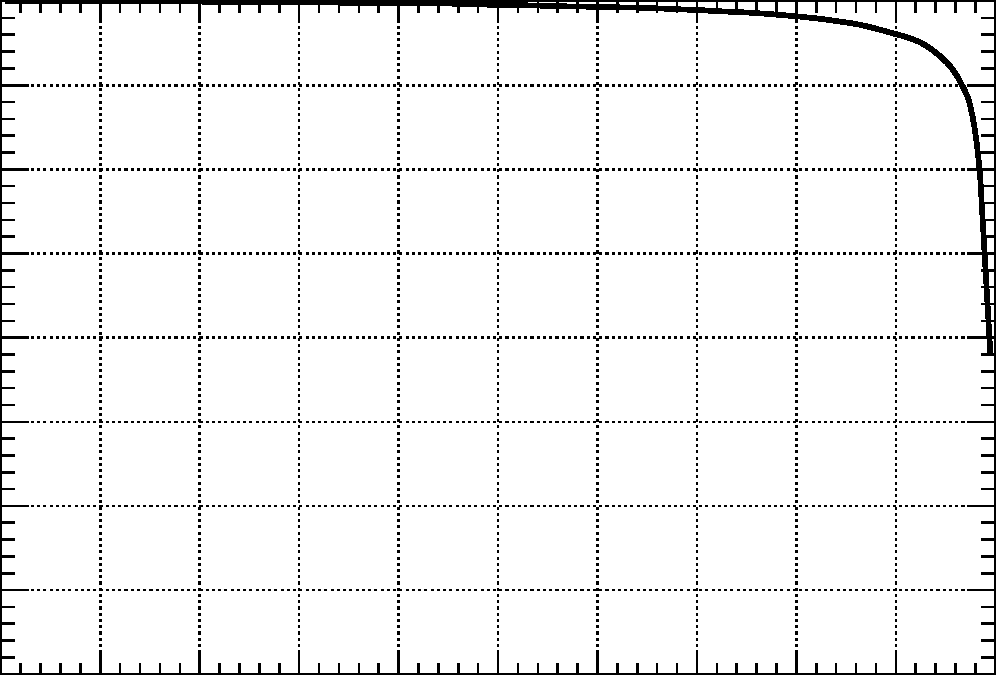
\includegraphics[width=0.9\textwidth]{BsDsK_TD/BDT/BDTG_RocCurve}};
        \begin{scope}[x={(image.south east)},y={(image.north west)}]
            \node at (0, -0.027) {\(0\)};
            \foreach \x in {1, ..., 10}
            {
                \tikzmath{\xtext = \x/10;}
                \node at (\x/10., -0.027) {\(\pgfmathprintnumber[fixed,precision=1,fixed zerofill=true]{\xtext}\)};
            }
            \foreach \y in {2, ..., 10}
            {
                \tikzmath{\ytext = \y/10; \ycoord = (\y - 1.97) / 8.07;}
                \node[anchor=east] at (0.005, \ycoord) {\(\pgfmathprintnumber[fixed,precision=1,fixed zerofill=true]{\ytext}\)};
            }
            \node[anchor=east] at (1.0, -0.10) {Signal efficiency};
            \node[rotate=90,anchor=east,inner xsep=0pt,outer xsep=0pt] at (-0.09, 1.0) {Background rejection};
        \end{scope}
    \end{tikzpicture}
    \caption{
        Example ROC~curve for the~BDT described in \cref{chp:BsDsK_TD_Data}, trained to separate \BsDsPi~events from combinatorial background.
        The black line parameterises a requirement on the classifier output, from very loose (top~left corner) to very tight (bottom~right corner).
        The optimal cutting point is somewhere in between, close to the top right corner.}
    \label{fig:methods_ROCCurve}
\end{figure}

\clearpage
\section{Particle identification}
\label{sec:PID}

The identification of particles~(PID) in~\lhcb is done by combining information from the~\rich, calorimeter and muon subdetectors.
However, since the efficiencies of correctly distinguishing pions, kaons, and protons are not well simulated, a data-driven method to determine the selection efficiency is warranted.

To determine the misidentification rate of pions and kaons, the decay \DstarDPi~is employed.
The pion originating directly from the \Dstarm~is labelled "S" to indicate that it is slow: due to the small mass difference between the \Dstarm~and \Dz~mesons there is only a small amount of phase space in the \Dstarm~decay, and so both the \Dz~and that pion are produced with low momenta in the \Dstarm~rest frame.
Identifying the slow pion by its momentum also allows identification of \Dz~decay products, using the charges of the respective tracks.
This allows unambiguous separation of pions and kaons using only tracking information, which can be used to calibrate the PID~efficiencies between pions and kaons from other subdetectors.

Similar to the procedure to calibrate the pion-kaon identification efficiency, the proton-pion efficiency can be calibrated, using the process \Lzppi.
Because of the mass difference between pions and protons, there is a momentum asymmetry between the decay products of \Lz~and \Lbar~baryons, which is exploited to distinguish the pion track from the proton track.

Each of these methods yields the efficiency of selecting a pion, kaon or proton for that specific decay.
However, different \bquark-hadron decays may have different properties.
In order to apply the efficiencies to such decays, they are computed as a function of track momentum, track transverse momentum, and number of tracks in the event.
An example of PID~efficiency as a function of kinematics can be seen in \cref{fig:Methods_PID_hist}.
Such a distribution can be used to calibrate the effect of a PID~requirement on a simulated sample, by reweighting the latter to the former.
Subsequently integrating also allows determining the total efficiency.
%
\begin{figure}[htb] \centerfloat
    \hspace*{-1cm}
    \begin{tikzpicture}
        \node[anchor=south west,inner sep=0] (image) at (0,0) {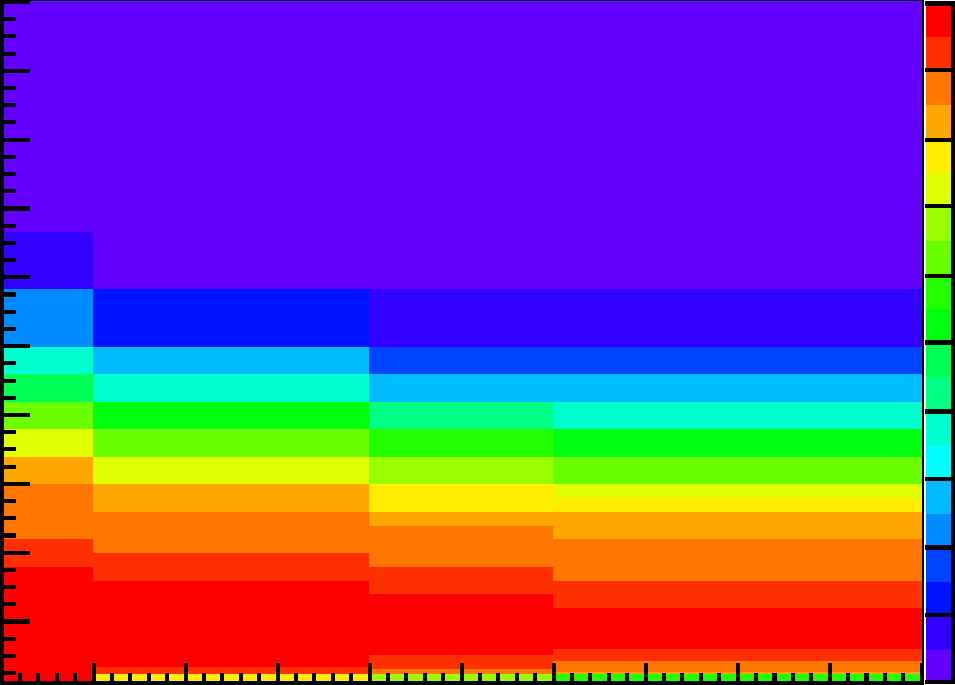
\includegraphics[width=0.9\textwidth]{methods/K_eff_PIDK5_2012_dw}};
        \begin{scope}[x={(image.south east)},y={(image.north west)}]
            \foreach \x/\xtext in {0, 50, ..., 500}
                \node at (\x/518, -0.025) {\(\xtext\)};
            \foreach \y/\ytext in {0, 20, ..., 200}
                \node[anchor=east] at (0.005, \y/201) {\(\ytext\)};
            \foreach \z in {0, ..., 10}
            {
                \tikzmath{\ztext = \z/10;}
                \node[anchor=west] at (1.0, 0.01 + \z/10.15) {\(\pgfmathprintnumber[fixed,precision=1,fixed zerofill=true]{\ztext}\)};
            }
            \node[anchor=east] at (1.0, -0.08) {Number of tracks in event};
            \node[rotate=90,anchor=east,inner xsep=0pt,outer xsep=0pt] at (-0.09, 1.0) {Track momentum [\si{\GeVc}]};
        \end{scope}
    \end{tikzpicture}
    \caption{
        Kaon selection efficiency for the requirement \({\dllkpi > 5}\), as a function of the number of tracks in the event (horizontal) and track momentum (vertical).
        These efficiencies are determined using decays of \Dstarm~mesons, following the data-driven method described in \cref{sec:PID}.
        The efficiency goes down as either the track momentum increases, which makes the distinction between pions and kaons by their speed harder; or as the track multiplicity increases, making Cherenkov ring reconstruction in the two~\rich{}es more difficult.}
    \label{fig:Methods_PID_hist}
\end{figure}

\clearpage
\section{Mass fits}
\label{sec:MassFits}

The yield of a specific signal decay is determined by performing a fit to the reconstructed invariant mass distribution of the final state.
Because mass is a unique property among hadrons, a peak in the mass distribution is attributed to decays of a particular parent hadron.
In order to perform a mass fit, several elements must be taken into account: signal, physics backgrounds, and combinatorial background.

\subsection{Signal}
\label{sec:MassFits_Signal}
The signal distribution takes the shape of a peak, centred around the mass of the parent hadron of interest.
Fundamentally, it takes the form of a Breit-Wigner shape, but the shape of relatively long-lived, weakly-decaying \bquark~hadrons in data is dominated by the resolution of the detector, which takes a Gaussian-like shape.
Additionally, radiation from the parent hadron causes a radiative tail to appear on the lower end of the mass spectrum.
The signal shape is parameterised using a double Crystal Ball~(DCB)~\cite{Skwarnicki:1986xj}, with a shared mean between the two Gaussian parts.
The central Gaussian functions describe the mass resolution, while the power-law tails account for the radiative tail on one side, and for events with poorly reconstructed mass on the other side.
The functional form of a DCB~shape is
%
\begin{multline} \label{eqn:Methods_DCB}
    \DCB(x; \DCBmu, \DCBsL, \DCBaL, \DCBnL, \DCBsR, \DCBaR, \DCBnR) = \\
    \begin{cases}
        \left(\dfrac{\DCBnL}{|\DCBaL|}\right)^{\DCBnL} e^{-\frac{1}{2}\DCBaL^2} \left[\dfrac{\DCBnL}{|\DCBaL|} - |\DCBaL| - \left(\dfrac{x - \DCBmu}{\DCBsL}\right)^{-\DCBnL}\right] &: \dfrac{x - \DCBmu}{\DCBsL} \leq \DCBaL \rlap{,} \\[3ex]
        e^{-\frac{1}{2} (x - \DCBmu)^2 / \DCBsL^2} &: \DCBaL\DCBsL < x - \DCBmu < 0 \rlap{,} \\[1ex]
        e^{-\frac{1}{2} (x - \DCBmu)^2 / \DCBsR^2} &: 0 > x - \DCBmu > \DCBaR\DCBsR \rlap{,} \\[1ex]
        \left(\dfrac{\DCBnR}{|\DCBaR|}\right)^{\DCBnR} e^{-\frac{1}{2}\DCBaR^2} \left[\dfrac{\DCBnR}{|\DCBaR|} - |\DCBaR| - \left(\dfrac{x - \DCBmu}{\DCBsR}\right)^{-\DCBnR}\right] &: \dfrac{x - \DCBmu}{\DCBsR} \geq \DCBaR \rlap{,}
    \end{cases}
\end{multline}
%
where \DCBmu~is the mean of the distribution, \DCBsLR~the widths of the central part left and right of~\DCBmu, \DCBaL~(\DCBaR) the distance to the left~(right) of~\DCBmu where the power-law tail starts, in units of \DCBsL~(\DCBsR), and \DCBnL~(\DCBnR) the slope of the left~(right) tail.
Often, the widths are taken to be equal, \({\DCBsL = \DCBsR = \DCBs}\), yielding a DCB with shared mean.
\Cref{fig:Methods_DCB_Examples} shows what such a distribution looks like. In general, a mass fit may have several signal components.
%
\begin{figure}[htb] \centerfloat
    \fontsize{9}{10.8}\selectfont
    \begin{subfigure}{.48\textwidth} \centerfloat
        \begin{tikzpicture}
            \node[anchor=south west,inner sep=0] (image) at (0,0) {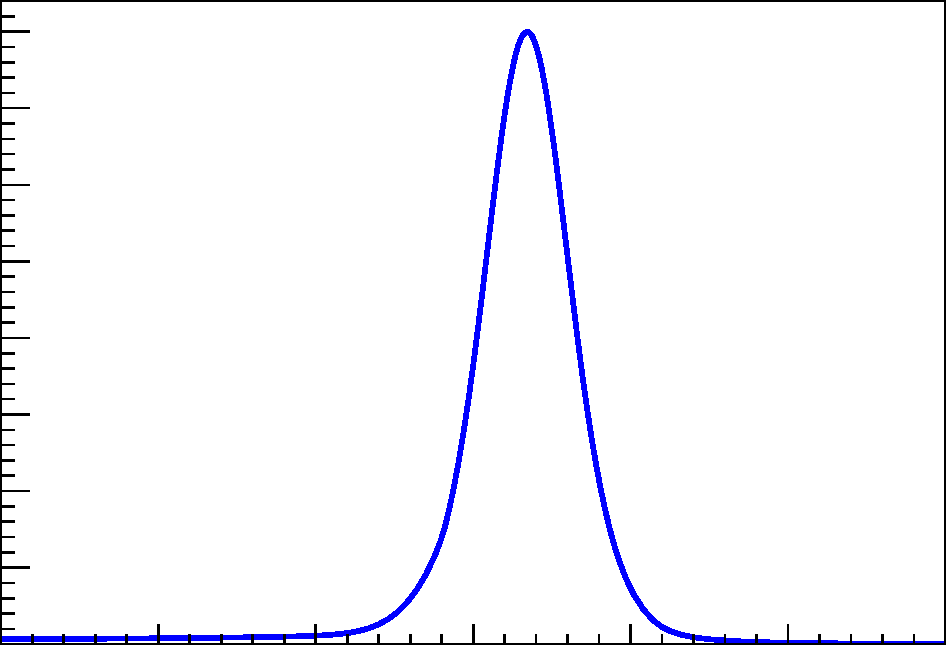
\includegraphics[width=0.9\textwidth]{methods/DCB_Example}};
            \begin{scope}[x={(image.south east)},y={(image.north west)}]
                \foreach \x in {0, ..., 6}
                {
                    \tikzmath{\xpos = (\x / 6); \xtext = 50 * \x + 5200;}
                    \node at (\xpos, -0.055) {\pgfmathprintnumber[fixed,precision=0,fixed zerofill=true,1000 sep={}]{\xtext}};
                }
                \node[anchor=east] at (1.0, -0.14) {\(x\)};
                \node[rotate=90,anchor=east,inner xsep=0pt,outer xsep=0pt] at (-0.07, 1.0) {\({\DCB(x)}\)};
            \end{scope}
        \end{tikzpicture}
    \end{subfigure} \hfill%
    \begin{subfigure}{.48\textwidth} \centerfloat
        \begin{tikzpicture}
            \node[anchor=south west,inner sep=0] (image) at (0,0) {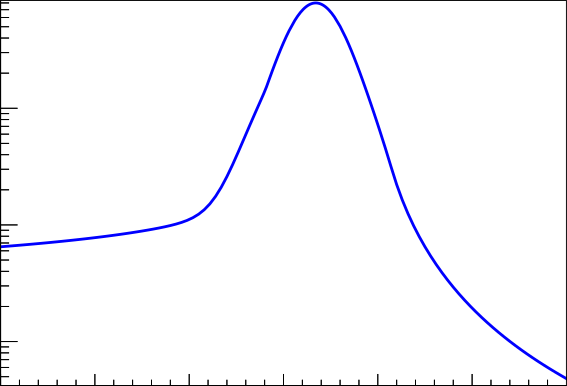
\includegraphics[width=0.9\textwidth]{methods/DCB_Example_log}};
            \begin{scope}[x={(image.south east)},y={(image.north west)}]
                \foreach \x in {0, ..., 6}
                {
                    \tikzmath{\xpos = (\x / 6); \xtext = 50 * \x + 5200;}
                    \node at (\xpos, -0.055) {\pgfmathprintnumber[fixed,precision=0,fixed zerofill=true,1000 sep={}]{\xtext}};
                }
                \node[anchor=east] at (1.0, -0.14) {\(x\)};
                \node[rotate=90,anchor=east,inner xsep=0pt,outer xsep=0pt] at (-0.07, 1.0) {\({\DCB(x)}\)};
            \end{scope}
        \end{tikzpicture}
    \end{subfigure}
    \caption{
        Example double Crystal Ball function, plotted in linear~(left) and logarithmic~(right) scale.
        The parameters are \({\DCBmu = \num{5367.11}}\), \({\DCBsL = \num{18.39}}\), \({\DCBsR = \num{11.43}}\), \({\DCBaL = \num{-2.19}}\), \({\DCBaR = \num{2.25}}\), \({\DCBnL = \num{2.37}}\), and \({\DCBnR = \num{0.42}}\), corresponding to the signal shape parameterisation used for \BsDsK, \DsmpPhiPi (see \cref{tab:BsDsK_TD_Signal_Shape_Results}) when \DCBmu~and \DCBsLR~are taken to be in units of~\si{\MeVcc}.
        Vertical units are omitted, as the normalisation is arbitrary.}
    \label{fig:Methods_DCB_Examples}
\end{figure}

\subsection{Physics backgrounds}
There are three distinguishable types of physics backgrounds: fully reconstructed backgrounds, partially reconstructed backgrounds, and misidentified backgrounds.
\begin{description}
\item[Fully reconstructed backgrounds] are decays with a different parent hadron but the same final state as the decay of interest.
    Their signal peak will be shifted with respect to that of the parent hadron, and therefore easily identifiable. These may very well be interesting in their own right, and may prompt further investigation.
\item[Partially reconstructed backgrounds] have the same final state as the parent hadron, apart from an extra decay product (such as a photon or a neutral pion), which is not accounted for in the reconstruction.
    The energy of the missing particle will also be absent in the invariant mass, which causes the distribution to be shifted to lower values, and smeared out. They have a shape which is difficult to model, and is generally extracted from simulation.
\item[Misidentified backgrounds] have a similar final state, but with a misidentified final-state particle.
    The shape of such a process is a smeared-out mass peak that is shifted with respect to that of the actual parent hadron.
\end{description}

Some backgrounds may belong to more than one category, such as partially reconstructed, misidentified backgrounds, or doubly partially reconstructed or doubly misidentified backgrounds.
These backgrounds have a small yield, so they do not have a large impact on a mass fit.

\subsection{Combinatorial background}
Combinatorial background results from random track combinations that happen to have an invariant mass close to that of the hadron of interest.
As such, these do not originate from any physical process, and the resulting distribution does not exhibit peaking structures.
It takes a negative exponential shape as a function of invariant mass, matching the number of random track combinations that can be made.
The exact parameters are difficult to determine from data, hence the usual strategy is to leave those parameters floating in the fit.

\subsection{Gaussian constraints}
If a parameter is known up to a certain uncertainty, such as the yield of a background process that can be calculated from prior information, it can be useful to constrain such a parameter in the mass fit.
One method to achieve that is to apply a Gaussian constraint to it.
This favours values for that parameter that are close to some predetermined mean value, as defined by a given width.
In a likelihood fit, such a constraint is taken into account by multiplying the likelihood by the deviation of the parameter value to that mean.
Multiple constraints can be taken into account, and the likelihood is multiplied with each.

\subsection{Kernel estimation} \label{sec:methods_KernelEstimation}
The shape of a distribution can often be taken directly from a representative simulated sample.
In order to use such a distribution in a mass fit, it must be transformed into a~PDF.
One way to achieve this is by using kernel estimation~\cite{Cranmer:2000du}.
This works by creating a Gaussian~function around each data point in the original distribution, adding those functions together, and normalising the resulting shape.
The width of the Gaussian~functions is a parameter that defines the smoothness of the resulting~PDF.

